\documentclass[11pt,a4paper]{article}
\usepackage[T1]{fontenc}
\usepackage[utf8]{inputenc}
\usepackage[czech]{babel}
\usepackage{lmodern}
\usepackage{geometry}
\usepackage{diagbox}
\geometry{top=27mm,bottom=20mm,left=22mm,right=22mm,headsep=7mm}
\usepackage{amsmath,amssymb,siunitx,graphicx,booktabs,longtable,array,float,caption,microtype,hyperref,xcolor,fancyhdr,enumitem}
\hypersetup{hidelinks}
\sisetup{output-decimal-marker={,},exponent-product=\cdot,per-mode=symbol}
\setlength{\parindent}{0pt}\setlength{\parskip}{4pt}
\captionsetup{font=small,labelfont=bf}
\captionsetup[table]{position=top,skip=6pt}
\captionsetup[figure]{position=bottom,skip=7pt}
\renewcommand{\arraystretch}{1.35}\setlength{\tabcolsep}{6pt}\setlength{\arrayrulewidth}{0.45pt}
\pagestyle{fancy}\fancyhf{}\setlength{\headheight}{25pt}
\fancyhead[L]{\footnotesize Pavel Pernička}
\fancyhead[C]{\footnotesize\bfseries Lab 2}
\fancyhead[R]{\parbox[b]{0.49\textwidth}{\raggedleft\footnotesize Dielektrické vlastnosti BaTiO$_3$}}
\fancyfoot[C]{\thepage}\renewcommand{\headrulewidth}{0.4pt}
\begin{document}
\section{Úloha 2a -- Dielektrické vlastnosti titaničitanu barnatého}
\subsection{Rozměry a geometrická kapacita}
Pro výpočty používáme rozměry $d=20\,\mathrm{mm}$ a $h=2{,}2\,\mathrm{mm}$ ze zadání. Geometrickou kapacitu vzorku určíme ze vztahu
\begin{equation}
C_0=\varepsilon_0\frac{\pi d^2}{4h}\qquad [\mathrm{F}].
\end{equation}
Po dosazení
\begin{equation}
C_0=8{,}854\cdot10^{-12}\frac{\pi(0{,}020)^2}{4\cdot0{,}0022}
\doteq1{,}264\cdot10^{-12}\,\mathrm{F}=1{,}264\,\mathrm{pF}.
\end{equation}

\subsection{Měření a výpočty}
Provedli jsme měření při teplotách $60$, $90$, $100$, $110$, $120$ a $130\,{}^\circ\mathrm{C}$. Oproti zadání jsme vynechali pokojovou teplotu, protože by ochlazování vzorku trvalo příliš dlouho. Pro každou teplotu jsme měřili při napětích $50$, $100$, $200$, $300$, $400$, $500$ a $600\,\mathrm{V}$.

Intenzitu elektrického pole jsme určili z napětí a tloušťky vzorku:
\begin{equation}
E=\frac{U_x}{h}\qquad [\mathrm{V/m}].
\end{equation}
Například při $U_x=100\,\mathrm{V}$:
\begin{equation}
E=\frac{100}{0{,}0022}\doteq45{,}45\,\mathrm{kV/m}.
\end{equation}

Z odečtených napětí $U_N$ a známé kapacity normálového kondenzátoru $C_N$ jsme stanovili kapacitu vzorku:
\begin{equation}
C_x=\frac{U_NC_N}{U_x}\qquad [\mathrm{F}].
\end{equation}
Například pro $U_x=100\,\mathrm{V}$, $U_N=165\,\mathrm{mV}$ a $C_N=4{,}25\,\mu\mathrm{F}$:
\begin{equation}
C_x=\frac{0{,}165\cdot4{,}25\cdot10^{-6}}{100}
=7{,}0125\cdot10^{-9}\,\mathrm{F}\doteq7{,}013\,\mathrm{nF}.
\end{equation}

Relativní permitivitu vypočítáme podle vztahu
\begin{equation}
\varepsilon'=\frac{C_x}{C_0}\qquad [-].
\end{equation}
Po dosazení nezaokrouhlených hodnot:
\begin{equation}
\varepsilon'=\frac{7{,}0125\cdot10^{-9}}{1{,}264375\cdot10^{-12}}
\doteq 5\,546\;[-].
\end{equation}

Ztrátový činitel už ale závisí na tvaru a ploše hysterezní smyčky, takže jeho hodnoty jsme vypočítali pomocí excelového sheetu, do kterého jsme vložili naměřené průběhy z osciloskopu. Všechny naměřené a vypočtené hodnoty jsou uvedeny v grafu níže.

\newpage

\subsection{Naměřené hodnoty}
V~tabulkách jsou uvedeny hodnoty pro teploty $60$ až $130\,{}^\circ\mathrm{C}$, tedy bez pokojové.
\begin{table}[H]\centering\caption{Naměřené napětí $U_N$ na normálovém kondenzátoru [mV].}\small\renewcommand{\arraystretch}{1.2}\setlength{\tabcolsep}{4pt}
\begin{tabular}{|c|r|r|r|r|r|r|}
\hline
\diagbox[width=7em,height=3em]{$U_x$ [V]}{$\vartheta$ [$^\circ$C]} & 60 & 90 & 100 & 110 & 120 & 130 \\ \hline
50 & 53 & 140 & 140 & 161 & 99 & 78 \\ \hline
100 & 165 & 356 & 365 & 342 & 198 & 160 \\ \hline
200 & 520 & 899 & 909 & 820 & 417 & 324 \\ \hline
300 & 966 & 1417 & 1433 & 1395 & 640 & 493 \\ \hline
400 & 1335 & 1879 & 1911 & 1975 & 883 & 657 \\ \hline
500 & 1691 & 2295 & 2332 & 2403 & 1102 & 826 \\ \hline
600 & 2068 & 2679 & 2765 & 2730 & 1304 & 985 \\ \hline
\end{tabular}\end{table}

\begin{table}[H]\centering\caption{Vypočtené hodnoty relativní permitivity $\varepsilon'$.}\small\renewcommand{\arraystretch}{1.2}\setlength{\tabcolsep}{4pt}
\begin{tabular}{|c|r|r|r|r|r|r|}
\hline
\diagbox[width=7em,height=3em]{$U_x$ [V]}{$\vartheta$ [$^\circ$C]} & 60 & 90 & 100 & 110 & 120 & 130 \\ \hline
50 & 3565 & 9444 & 9444 & 10861 & 6679 & 5262 \\ \hline
100 & 5565 & 12008 & 12312 & 11536 & 6679 & 5397 \\ \hline
200 & 8770 & 15162 & 15330 & 13829 & 7033 & 5464 \\ \hline
300 & 10861 & 15932 & 16112 & 15685 & 7196 & 5543 \\ \hline
400 & 11257 & 15845 & 16115 & 16654 & 7446 & 5540 \\ \hline
500 & 11408 & 15482 & 15732 & 16211 & 7434 & 5572 \\ \hline
600 & 11626 & 15061 & 15544 & 15347 & 7331 & 5537 \\ \hline
\end{tabular}\end{table}

\begin{table}[H]\centering\caption{Vypočtené hodnoty ztrátového činitele $\mathrm{tg}\,\delta$.}\small\renewcommand{\arraystretch}{1.2}\setlength{\tabcolsep}{4pt}
\begin{tabular}{|c|r|r|r|r|r|r|}
\hline
\diagbox[width=7em,height=3em]{$U_x$ [V]}{$\vartheta$ [$^\circ$C]} & 60 & 90 & 100 & 110 & 120 & 130 \\ \hline
50 & 0,445 & 0,458 & 0,475 & 0,205 & 0,165 & 0,172 \\ \hline
100 & 0,550 & 0,463 & 0,415 & 0,253 & 0,155 & 0,155 \\ \hline
200 & 0,511 & 0,419 & 0,377 & 0,267 & 0,162 & 0,164 \\ \hline
300 & 0,482 & 0,371 & 0,332 & 0,268 & 0,162 & 0,169 \\ \hline
400 & 0,440 & 0,342 & 0,309 & 0,251 & 0,161 & 0,169 \\ \hline
500 & 0,381 & 0,318 & 0,292 & 0,227 & 0,161 & 0,166 \\ \hline
600 & 0,353 & 0,296 & 0,274 & 0,213 & 0,163 & 0,171 \\ \hline
\end{tabular}\end{table}

\subsection{Grafické závislosti}
\begin{figure}[H]\centering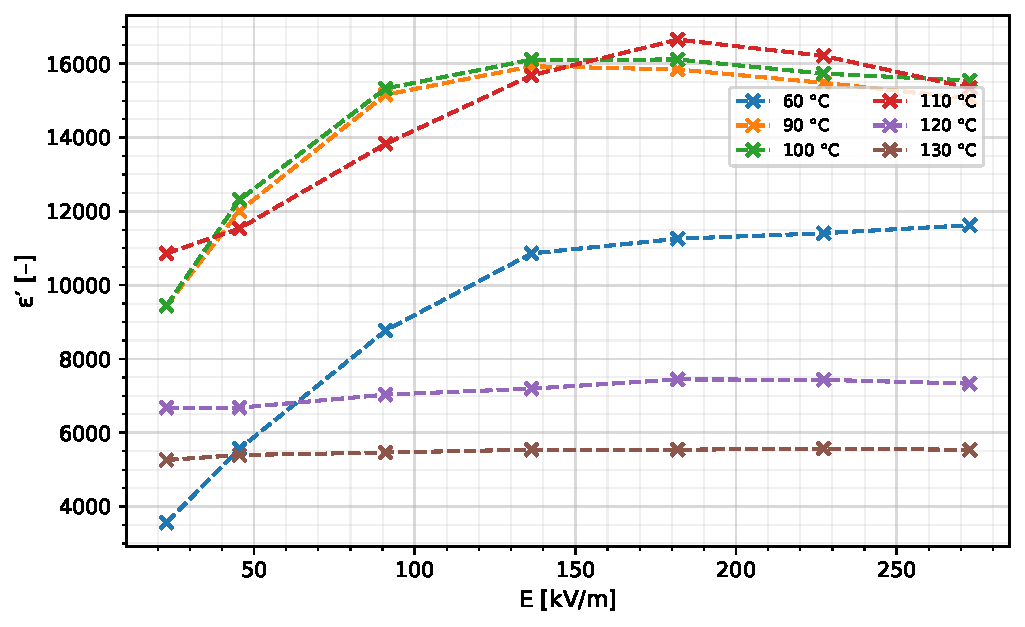
\includegraphics[width=0.91\linewidth]{graf_permitivita.pdf}\caption{Závislost relativní permitivity $\varepsilon'$ na intenzitě elektrického pole $E$ při různých teplotách.}\end{figure}
\begin{figure}[H]\centering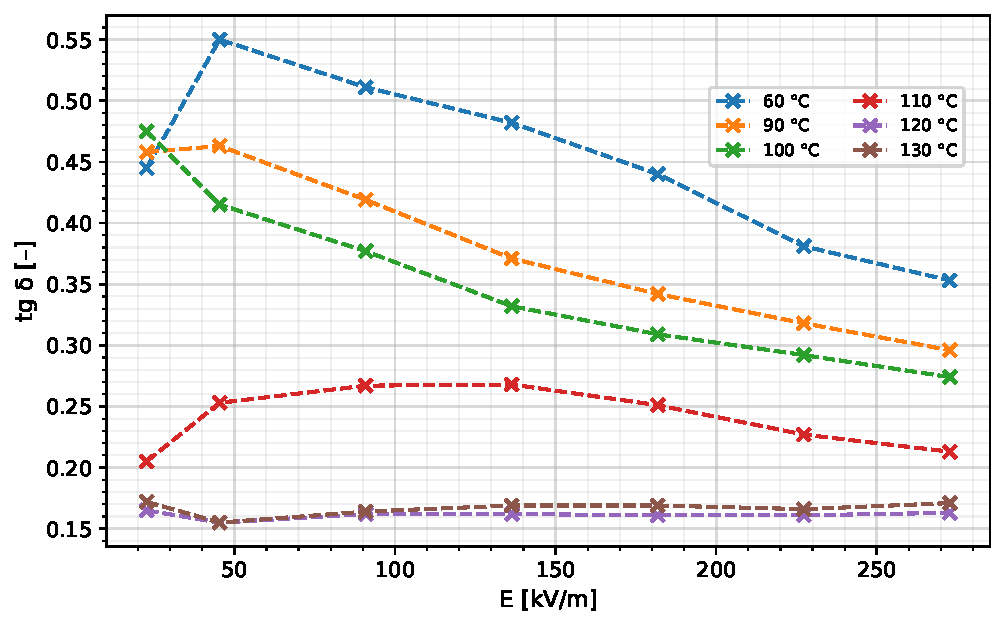
\includegraphics[width=0.91\linewidth]{graf_ztraty.pdf}\caption{Závislost ztrátového činitele $\mathrm{tg}\,\delta$ na intenzitě elektrického pole $E$ při různých teplotách.}\end{figure}

\newpage
\section{Úloha 2b -- Součinitel nelinearity BaTiO$_3$}
\subsection{Výpočet součinitele nelinearity}
Pro stanovení nelinearity používáme hodnoty relativní permitivity z~úlohy 2a.

Součinitel nelinearity je definován jako
\begin{equation}
K=\frac{\varepsilon'_{\max}}{\varepsilon'_{\mathrm{poč}}}\ [-].
\end{equation}

Počáteční a maximální permitivitu určíme z grafu závislosti $\varepsilon' = F(E)$ v našem omezeném měřícím rozsahu.

Například pro $100\,{}^\circ\mathrm{C}$ je to z~tabulky v~úloze 2a:
\begin{equation}
\varepsilon'_{poč}=12\,312,\qquad \varepsilon'_{\max}=16\,115,
\end{equation}
z čehož po dosazení dostaneme
\begin{equation}
K_\mathrm{měř}=\frac{16\,115}{12\,312}\doteq1{,}309.
\end{equation}
\begin{table}[H]\centering\caption{Počáteční a max. relativní permitivity a vypočtený součinitel nelinearity v~intervalu 100--600~V.}\small
\begin{tabular}{|r|r|r|r|}\hline
$\vartheta$ [$^\circ$C] & $\varepsilon'_{poč}$ [--] & $\varepsilon'_{\max}$ [--] & $K_\mathrm{měř}$ [--] \\\hline
60 & 5565 & 11626 & 2,089 \\ \hline
90 & 12008 & 15932 & 1,327 \\ \hline
100 & 12312 & 16115 & 1,309 \\ \hline
110 & 11536 & 16654 & 1,444 \\ \hline
120 & 6679 & 7446 & 1,115 \\ \hline
130 & 5397 & 5572 & 1,032 \\ \hline
\end{tabular}\end{table}

\begin{figure}[H]\centering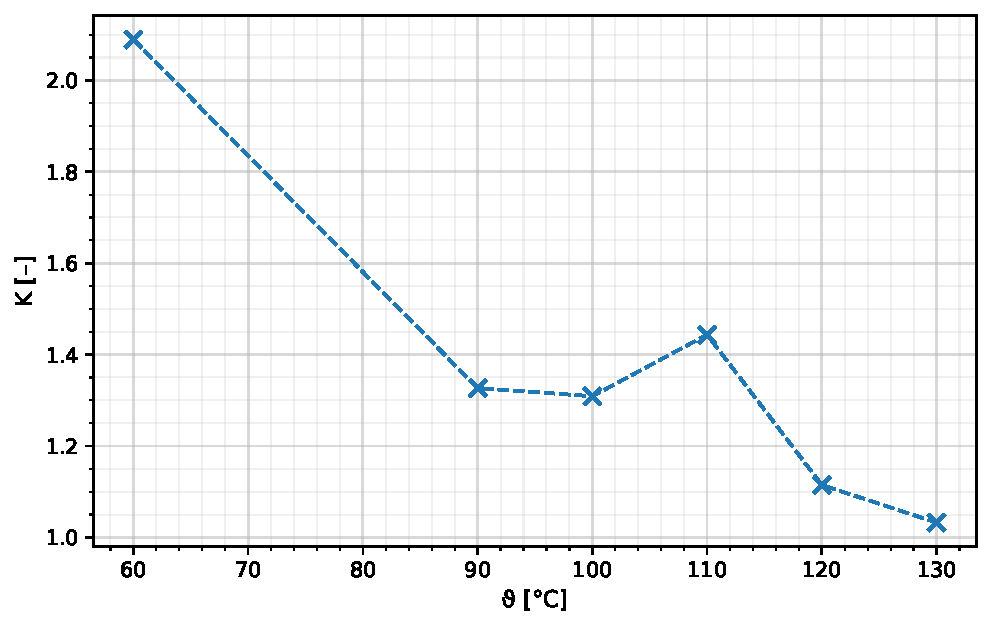
\includegraphics[width=0.88\linewidth]{graf_nelinearita.pdf}\caption{Teplotní závislost součinitele nelinearity stanoveného z~měřeného intervalu 100--600~V.}\end{figure}



\section{Závěr}

\subsection{Vyhodnocení úlohy 2a}

Měřením jsme zjistili, že relativní permitivita
BaTiO$_3$ výrazně závisí na intenzitě elektrického
pole a~hlavně teplotě. Při teplotách 60 až 110~$^\circ$C
permitivita s rostoucí intenzitou nejprve rostla
a následně dosahovala maxima nebo začala pomalu klesat.
Nejvyšší hodnotu $\varepsilon'=16\,654$ jsme
naměřili při 110~$^\circ$C a napětí 400 V.
To odpovídá teoretickému očekávání, protože
s rostoucí intenzitou pole dochází k přeskupování
domén a zvyšování polarizace. Po dosažení
polarizačního nasycení se již polarizace výrazně
nezvyšuje, a relativní permitivita proto klesá.

Při teplotách 120 a 130 $^\circ$C jsme pozorovali
výrazný pokles permitivity a její závislosti na
intenzitě pole. To souvisí s Curieho teplotou,
která je u BaTiO$_3$ přibližně 120 $^\circ$C.
Při jejím překročení se tetragonální struktura
mění na kubickou a zaniká spontánní polarizace.
Z materiálu se stává paraelektrikum.

Ztrátový činitel byl nejvyšší při nižších teplotách
a s rostoucí intenzitou elektrického pole většinou
klesal. Při 60 a 110 $^\circ$C však nejprve vzrostl
a až poté začal klesat. Nejvyšší hodnotu
$\mathrm{tg}\,\delta=0{,}550$ jsme naměřili
při 60 $^\circ$C a napětí 100 V.

Při 120 a 130 $^\circ$C se ztrátový činitel
pohyboval přibližně mezi 0,155 a 0,172
a na intenzitě pole téměř nezávisel.
To souvisí opět s přechodem materiálu do
paraelektrického stavu v okolí Curieho
teploty.

\subsection{Vyhodnocení úlohy 2b}

Součinitel nelinearity vykazoval až na teplotu 110 $^\circ$C
výraznou teplotní závislost. Nejvyšší hodnotu
$K_\mathrm{měř}=2{,}089$ jsme stanovili
při 60 $^\circ$C. S rostoucí teplotou
součinitel převážně klesal, až při
130 $^\circ$C dosáhl hodnoty 1,032.

Pokles součinitele souvisí s přechodem
materiálu z feroelektrického do
paraelektrického stavu v~okolí Curieho
teploty. Nad touto teplotou zaniká
spontánní polarizace a relativní
permitivita je na intenzitě elektrického
pole tím pádem závislá výrazně méně.

V zadání jsou pro BaTiO$_3$ uvedeny
typické hodnoty součinitele nelinearity
3 až 4, naše výsledky jsou tedy nižší.
Počáteční permitivitu jsme však
nestanovovali při velmi malých intenzitách
pole, ale použili jsme minimální hodnotu
z intervalu 100 až 600 V.

\end{document}
